%%%%%%%%%%%%%%%%%%%%%%%%%%%%%%%%%%%%%%%%%%%%%%%%%%%%%%%%%%%%%%%%%%%%%%
\section{Physics Requirements for Calibration}
\label{sec:calibphys} %% 3 pages

DUNE has a broad physics program which includes long baseline physics, supernova physics, nucleon decay and other exotic searches. The physics processes which lead to the formation of these signals and the detector effects which impact their propagation must be carefully understood in order to perform adequate calibrations as it ultimately impacts the detector's energy response. In addition to measurements of specific detector effects, studies that address energy resolution performed with various sources offer a higher level evaluation of detector performance which can be used to assess the impact on physics analyses and\slash or verify specific aspects of the detector response model relevant for that physics.

In addition to calibration, several other categories of effects can impact long baseline physics such as the neutrino interaction model, insufficient calibration, or reconstruction pathologies. For this note, we take as a target that calibration, by itself, needs to be sufficient for DUNE's program; other issues which limit the physics program are out of scope and can only amplify the overall error budget. Section~\ref{sec:lbl} describes the calibration-driven physics requirements for the long baseline program, Section~\ref{sec:sn} describes the supernova physics program which relies on low-energy interactions, and Section~\ref{sec:exotica} describes exotic physics model searches, including nucleon decay. 

%Most of the studies done so far are generic, that is they demonstrate the impact of categories of effects. For example, the impact of energy bias is discussed for the long baseline analysis, and such bias can stem from: the neutrino interaction model, insufficient calibration, or reconstruction pathologies. For this note, we take as a target that calibration, by itself, needs to be sufficient for DUNE's program; other issues which limit the physics program are out of scope and can only amplify the overall error budget.
%errors always add in quadrature. 
 
%%%%%%%%%%%%%%%%%%%%%%%%%%%%%%%%%%%%
\subsection{Long-baseline physics }\label{sec:lbl}
%- Kendall (first pass) and Sowjanya}

DUNE's \dword{lbl} program %long baseline program (LBL) 
uses measurements of % $\nu_e$, $\overline{\nu}_e$ 
\nue, \anue appearance and \numu %$\nu_\mu$ 
disappearance, to probe for new physics with neutrinos, including a search for CP violation (\dword{cpv}), and the mass hierarchy. Additional far detector physics includes measurements with atmospheric neutrinos, $\nu_\tau$ appearance, and non-standard matter  interactions or other effects. These programs all
rely on neutrinos of energies 0.2-10 GeV. 

In the physics volume of the DUNE CDR~\cite{Acciarri:2015uup}, Figure~3.23 shows that increasing the uncertainties on the \nue event rate from 
\num{2}\% overall\footnote{This uncertainty is an uncorrelated normalization uncertainty on the far detector \nue rate in a four sample FD fit that assumes reasonable near detector constrains on flux and cross sections.} to \num{3}\% results in a \num{50}\% longer run period, 
The CDR also assumes that the fiducial volume is understood at the 1\% level. Thus, calibration information needs to provide approximately 1-2\% understanding of normalization, energy and position resolution within the detector. Later studies~\cite{ebias} expanded the simple treatment of energy  presented above. In particular, \num{1}\% bias on the lepton energy has a significant impact on the sensitivity to \dword{cpv}. A \num{3}\% bias in the hadronic state (excluding neutrons), is important as well, as the Bjorken $y$ distribution for neutrinos and antineutrinos are quite different, and a larger fraction of the  antineutrino's energy will go into the hadronic state.  Finally, while studies largely consider a single, absolute energy scale, relative spatial differences across the enormous DUNE \dword{fd} volume will need to be monitored and corrected; this is also true for changes which occur in time. 

Some of the primary requirements for \dword{lbl} physics include neutrino vertex reconstruction, particle identification, electromagnetic shower energy measurement, e/$\gamma$ separation, and momentum measurements (e.g. using particle range or Multiple Coulomb Scattering). A number of in-situ calibration sources will be required to address these broad range of requirements. Michel electrons, neutral pions and radioactive sources (both intrinsic and external) are valuable for calibrating detector response to electromagnetic activity in the tens to hundreds of MeV energy range. Stopping protons and muons from cosmic rays or beam interactions form an important calibration source for calorimetric reconstruction and particle identification.
\Dword{protodune}, as a dedicated test beam experiment, provides critical measurements to characterize and validate particle identification strategies in a 1~kt scale detector and will be an essential input to the overall program. 
Dedicated calibration systems, like laser-based ones, can provide in-situ full volume measurements of electric field distortions. The electric field is a critical aspect of calibration, as  estimates of calorimetric response and particle identification depend on electric field through recombination. 

Spatial deformations within the detector  can also impact the energy estimator. Particles in the detector will repeatedly (elastic) Coulomb scatter with the liquid resulting in small, randomized deviations to their path. Multiple Coulomb Scattering (MCS) is used estimate the particles initial energy, but relies on a known distance the particles traveled. If the  distance is different than expectation due to misalignments or spatial deformations caused by electric field, then this may bias the estimator. The stringent physics requirements on energy scale and fiducial volume also put similarly stringent requirements on detector physics quantities such as electric field, drift velocity, electron lifetime, and the time dependences of these quantities.

The calibration group in conjunction with the \dword{lbl}, Simulation and Reconstruction groups will develop the necessary tools to propagate detector physics effects into \dword{lbl} physics. Some of the studies planned include quantifying (at truth level) the impact of drift field distortions (due to ionization and non-ionization sources such as misalignment) on muon, electron, pion, and proton tracks. The impact should also be assessed for overall calorimetry including below particle tracking or ID threshold. Also,  quantifying the relative importance of electromagnetic shower photons below pair production threshold will be pursued. %and understand the impact for DUNE.

%The ionization signal received at the anode ($dQ/dx$) depends on~\cite{ARGONEUTrecomb}:

%\begin{equation}
%dQ/dx = dE/dx \times \frac{1}{W} \times R \times L \times D \times C
%\end{equation}
% FOrumula from J. Klein talk at Aug 2017 CM: https://indico.fnal.gov/event/13293/session/12/contribution/90/material/slides/0.pdf

%where $dE/dx$ is the energy lost by the particle initially through ionization over a distance $dx$, $W$ is the energy needed to free an electron, $R$ is the recombination factor of electrons with Ar${^+}$ ions, $L$ is the drift-lifetime of electrons, $D$ is electron diffusion constant, and $C$ is the calibration of electronics response. For a particle not traveling parallel to any wire, $dx = |dy+dz+v_d t|$, where $dy$ and $dz$ are the distances in the $y$ and $z$ directions, and the $x$ (drift) direction position depends on the drift velocity ($v_d$) and drift time ($t$).

%SG: the above equation and related description is moved to David's section.

%The electric (E) field  has a critical role in the DUNE as the E field impacts drift velocity, recombination, and therefore the energy estimate ($dQ/dx$). Approximately, a \num{1}\% distortion to the E field will correspond to a \num{0.25}\% distortion to $dQ/dx$. Distortions of the E field can occur locally or globally, and are due to a variety of effects. For example, \dword{cpa} misalignment,  \dword{cpa} structural deformations, and APA/CPA offsets  may create E field distortions localized in space. Non-uniform resistivity in the voltage dividers which create the E field may create a net E field distortion localized in space, and a failure of a resistor will create a sudden change in time. Penetrations to the field cage will also create distortions to the E field. Finally, accumulation of slow moving positive ions, created from cosmic rays or from Ar39 localized in space (``space charge'') will distort the E field. Each individual E field distortion sources may add in quadrature with other effects, and can exceed \numrange{1}{4}\,\% overall E field distortion.
%We note that if DUNE does not run at nominal E field, then recombination is higher, and the drift time is longer. Both of these effects make the understanding of E field in-situ even more important. Distortions to the electric field also create spatial deformations which propagate to $dQ/dx$. Examples of this include space charge, and misalignments. These distortions occur in three dimensions, but the dominant effect is in the drift direction (the direction of the nominal E field, $x$), so for this document, we estimate the scale of these effects only in $x$.

%SG: most of the above discussion is now in the laser section to motivate the laser more strongly. This is replaced in this section by a more generic description of how things happen.

%Spatial deformations within the detector  can also impact the energy estimator. Particles in the detector will repeatedly (elastic) Coulomb scatter with the liquid resulting in small, randomized deviations to their path. Multiple Coulomb Scattering (MCS) is used estimate the particles initial energy, but relies on a known distance the particles traveled. If the  distance is different than expectation due to misalignments or E field spatial deformations, then this may bias the estimator. % http://meroli.web.cern.ch/meroli/lecture_multiple_scattering.html
%SG: the above is moved to the main section right after E-field is discussed.

%The fiducial volume (and position resolution) is impacted by our understanding of the distances within the detector, drift velocity and electric field. Like the energy scale case, fiducial volume is affected by relative distortions across the detector either from spatial or temporal causes.
%The drift Drift distance -> Drift velocity affects FV via formula. Spatial distortions also affect MCS, FV.
%The stringent physics requirements on energy scale and fiducial volume therefore put similarly stringent requirements onto E field, spatial deformations (alignment), drift velocity, electron lifetime, and the time dependences of these quantities.

%The remaining studies to clarify the role of calibration planned in conjunction with the long baseline program are:
%\begin{itemize}
%\item Quantify the distortion (at truth level quantities) on muon, electron, pion, proton tracks from E field distortions, misalignment, and other known effects which calibration probes. The impact should also be assessed for overall calorimetry (below particle tracking or ID threshold). 
%\item Quantify the relative importance of electromagnetic shower photons below pair production threshold. %Not sure what the current outlook on this is, but last I heard (4-5 years ago) it would limit electron energy calibration to ~6-7%, even if everything else was perfect.

%\end{itemize}

\subsection{Supernova physics }
\label{sec:sn}

The DUNE Supernova burst and low-energy (\dword{snble}) neutrino physics focuses on physics that can be done with neutrinos with energies of less than about \SI{100}{\MeV}. The primary physics topic is detection of the burst of neutrinos from a core-collapse supernova, with potentially very rich physics and astrophysics yield. The expected signal is a burst of neutrinos of all flavors in the few- to few-tens-of-\si{\MeV} range within tens of seconds, of which the component detectable by the DUNE LArTPC is primarily $\nu_e$. Overall, one wants to know the energy, flavor and time structure of the burst. The \dword{snble} physics also considers solar neutrinos (energies up to $\sim$\SI{15}{\MeV}) and the diffuse supernova neutrino flux (\dword{dsnb}) which should have roughly similar properties to the \dword{snb} flux, but much lower rate. For the latter two physics topics, the main concern is the background. 

These events present specific reconstruction and calibration challenges. Supernova neutrino events, due to their low energies, will manifest themselves as small, perhaps few tens of \si{\cm}, stub-like tracks from electrons (or positrons from the rarer \anue interactions). Events from \nue charged-current interactions, $\nu_e+{}^{40}{\rm Ar}\rightarrow e^{-}+{}^{40}{\rm K}^{*}$, are likely to be accompanied by de-excitation products -- gamma rays and/or ejected nucleons, as shown in Figure~\ref{fig:SNBspectrum}. Gamma-rays are in principle observable via energy deposition from Compton scattering, which will show up as small charge blips in the \dword{tpc}. Ejected nucleons may result in loss of observed energy for the event. Elastic scattering on electrons will result in single
scattered electrons, and single gamma rays may result from \dword{nc} excitations of the argon nucleus.  Each event category has, in principle, a distinctive signature. In each case, observable energy is shared between different charge clusters and types of energy depositions.  

\begin{dunefigure}[]{fig:SNBspectrum}{Expected SNB electron neutrino energy spectrum and contributions of emitted particle types to the visible energy.}
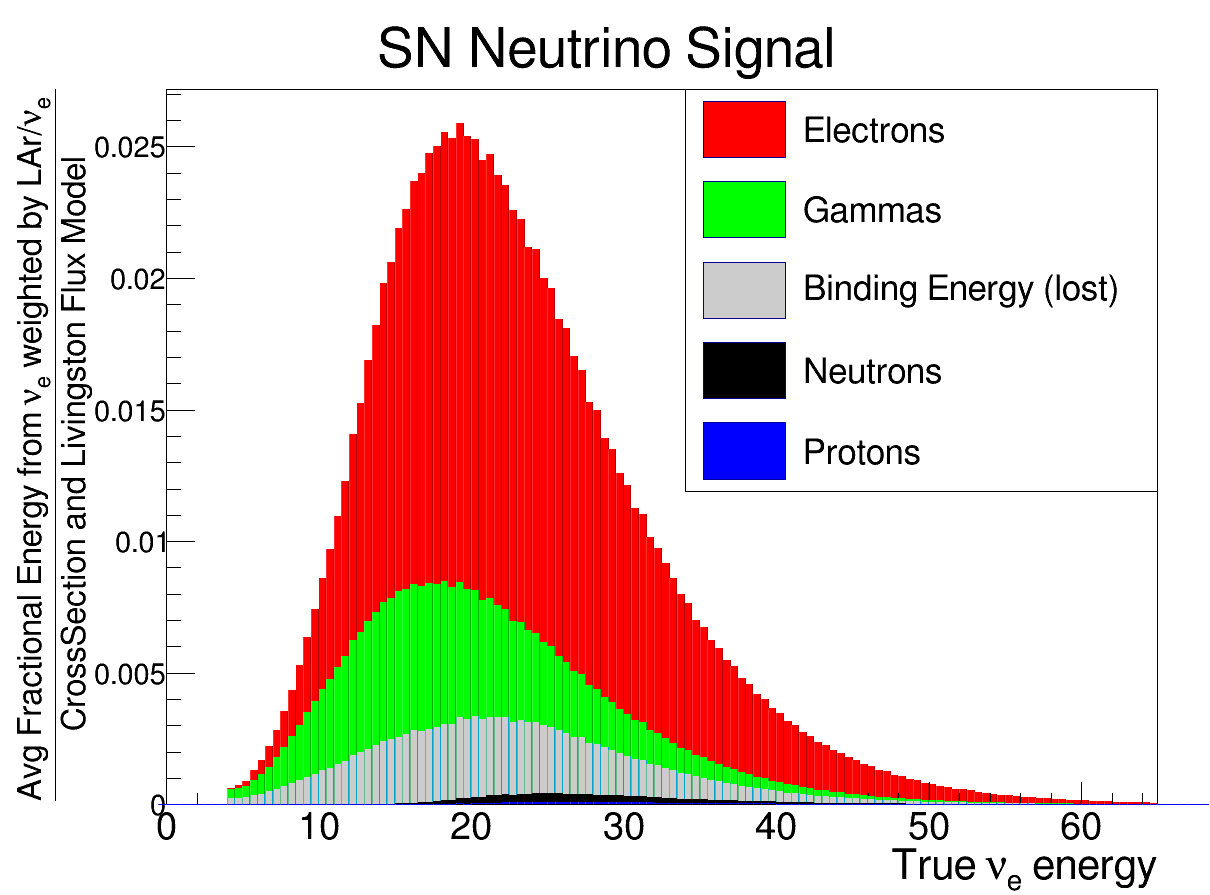
\includegraphics[height=2.0in]{snb-spectrum.png}
\end{dunefigure}

The canonical reconstruction task is to identify the interaction channel, the neutrino flavor for \dword{cc} events, and to determine the four-momentum of the incoming neutrino; this overall task is the same for low-energy events as for high-energy ones.  The challenge is to reconstruct the properties of the lepton (if present), and to the extent possible, to tag the interaction channel by the pattern of final-state particles.

Calibration of absolute energy scale and understanding of energy resolution will be important for interpretation of the signal. We expect nominally $\sim$\num{20}\% resolution, although better would be desirable for resolution of supernova spectral features. Furthermore, a sample of data events of known properties with which to validate efficiencies of selection and reconstruction algorithms would be very valuable.

Given that the signal is expected to be uniformly distributed within the detector, absolute position resolution may not be critical (and events are likely to be widely separated in space for all but the very closest supernovae). However, good position resolution of photon detection is needed for good energy resolution, via correction for attenuation of charge during drift. Photon detectors in general may provide useful trigger information (and perhaps also ancillary energy information), so calibration of their time and light response is mandatory.

Absolute timing of events will be important for tracking the time structure of the burst. We expect that some $\sim$\num{0.1} fraction of a drift time ($<$\si{\ms}) will be sufficient for sensitivity to interesting physics signatures which vary in time. Therefore calibration of absolute timing response will be of value.

Understanding of backgrounds is also critical for reconstruction of low energy events, and for setting detector requirements. Small single-hit blips from $^{39}$Ar or other impurities may fake de-excitation gammas and also affect triggering. Backgrounds may be especially important for photon detectors.  Understanding of detector response to radiological backgrounds will therefore also be of value.

Potential calibration sources in this energy range include Michel electrons (studied in \dword{microboone}~\cite{Acciarri:2017sjy}), which have a well known spectrum up to $\sim$50~MeV. One can also calibrate using $\gamma$, $\beta$ or neutron sources (both intrinsic and external), which primarily give access to energies less than about 10~MeV. It is more challenging to find ``standard candles'' between 50~MeV and $\sim$\SI{100}{\MeV}, beyond cosmic-ray muon energy loss. \Dword{protodune} could potentially be a test bed for various calibration strategies. One can imagine also ancillary studies of detector response using detectors such as LArIAT~\cite{Cavanna:2014iqa}, \dword{microboone}~\cite{Acciarri:2016smi}, and SBND~\cite{Antonello:2015lea}. The ultimate calibration would be using a source of neutrinos from pion decay at rest, such as that available at the Spallation Neutron Source~\cite{Bolozdynya:2012xv}, which have energies up to \SI{50}{\MeV} with a well-understood spectrum.

%%%%%%%%%%%%%%%%%%%%%%%%%%%%%%%%%%%%
\subsection{Exotic Physics}\label{sec:exotica}

Nucleon Decay and other exotic physics calibration needs are comparable to the \dword{lbl} program as listed in Section~\ref{sec:lbl}. Signal channels for light dark matter and sterile neutrino searches will be neutral current interactions which are background to the \dword{lbl} physics program. The nucleon decay group has done studies of detection of the proton decay channel \ptoknubar, %$p\rightarrow K+ \overline{\nu}$, 
where the kaon decays to a muon and then a positron~\cite{protondecaywidths}. Based on the widths of $dE/dx$-based metrics of particle identification, qualitatively, we need to calibrate $dE/dx$ across all drift and track orientations at the few percent level or better, which is a similar target of interest as the \dword{lbl} effort.

%%%%%%%%%%%%%%%%%%%%%%%%%%%%%%%%%%%%

%KM notes: The Low Energy physics program includes searches for proton decay, detection of a core collapse supernova and signatures of dark matter.
%Many of the concerns of the low energy program are shared with  long baseline program, especially time dependent effects and identification of few MeV interactions. For example, supernova neutrinos have energies of about 20 MeV, but the energy is shared between neutron interactions, re-scattering of the electron, and de-excitation photons. So, a 20 MeV neutrino may be the combination of four 5 MeV sub-events. 
%The supernova (and other low energy physics) programs may have less stringent requirements (??10\% energy, position resolution??) but may be more susceptible to threshold effects.
